% In the previous chapter, we showed that voltage and current appear in form of waves on transmission lines and that the properties of this traveling wave are governed by the propagation constant, $\gamma$. 
Now, let us try to understand the physical significance of this complex quantity $\gamma$.

\section{The complex quantity $\gamma$}\label{lec:lec3}
From equation~\eqref{eqn:deqn}, we have established that $\gamma$ is given as
\begin{dmath}
\gamma = \sqrt{(R + \jmath\omega L)(G + \jmath\omega C)}
= \alpha + \jmath\beta
\label{eqn:gamma}
\end{dmath}
Where $R$ is the resistance per unit length, $L$ is the inductance per unit length, $G$ is the conductance per unit length, and $C$ is the capacitance per unit length.

For the forward traveling wave in equation~\eqref{eqn:solnv}, we can express it in phasor form as follows
\begin{equation}
V^+e^{-\gamma x} =\left|V^+\right|e^{-(\alpha + \jmath\beta)x}e^{\jmath\phi}
\end{equation}
If we assume $V^+$ is real and have an initial phase $\phi = 0$, then;
\begin{dmath}
V^+e^{-\gamma x} = \left| V^+\right| e^{-(\alpha + \jmath\beta)x}e^{\jmath0}\quad\text{But }e^{j0}\text{ = }e^0\text{ = }1
= \left| V^+\right| e^{-\alpha x}e^{-\jmath\beta x}
\label{eqn:phasorforward}
\end{dmath}
Equation~\eqref{eqn:phasorforward} is the phasor representation.

In phasor representation, the time varying part is ignored so the complete expression for $V^+$ is 
\begin{equation*}
V^+ = \left|V^+\right|e^{j(\omega t + \phi)} e^{-\gamma x} 
\end{equation*}
and the phasor form like equation~\eqref{eqn:phasorforward} with initial phase $\phi$ is
\begin{equation*}
V^+ = \left|V^+\right|e^{j\phi} e^{-\gamma x}
\end{equation*}

\subsection{The Phase constant}\index{phase constant}
From the equation~\eqref{eqn:phasorforward}, we see that as the wave propagates i.e as the value of x increases, the quantity $\left|V^+\right|e^{-\alpha x}$ is exponentially decreasing while $e^{-\jmath\beta x}$ is the sinusoidal part that oscillates because according to \footnote{
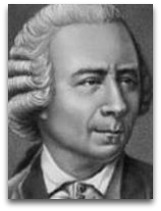
\includegraphics[scale=0.2]{./graphics/euler}

Leonhard Euler (15 April 1707 - 18 September 1783). He was an 18th-century Swiss mathematician and physicist who made significant contributions to various branches of mathematics and introduced numerous concepts that are widely used today. He was born on April 15, 1707, in Basel, Switzerland, and spent the majority of his career in St. Petersburg, Berlin, and Basel.

Euler's work spanned diverse areas of mathematics, including calculus, number theory, graph theory, and differential equations. He made groundbreaking contributions to each of these fields, revolutionizing the way mathematicians approached and solved problems. Euler's extraordinary output includes over 850 published papers, covering a vast range of mathematical topics.

One of Euler's most famous achievements is the Euler's formula, also known as Euler's identity or Euler's equation. The formula relates five fundamental mathematical constants: e (the base of natural logarithms), $\pi$ (pi, the ratio of a circle's circumference to its diameter), $i$ (the imaginary unit, which satisfies $i^2 = -1$), 1 (the multiplicative identity), and 0 (the additive identity). The formula can be written as:
\begin{align*}
e^(i\pi) + 1 = 0.
\end{align*}

Euler's formula connects exponential functions, complex numbers, and trigonometry in a profound way. It highlights the unexpected relationship between these seemingly unrelated mathematical concepts. The formula has been hailed as one of the most beautiful equations in mathematics due to its elegant simplicity and deep significance.
}Euler's formula $e^{-\jmath\beta x} = \cos{\beta x} - \jmath \sin{ \beta x}$. Hence phase (spatial phase) is obtained from $e^{-\jmath\beta x}$.

We now see that the equation~\eqref{eqn:gamma} has $\alpha$ that controls the amplitude of the wave as we move in the x-direction and $\beta$ that controls the phase of the wave along the transmission line. Hence,
\begin{equation}
\text{Spatial phase} = -\jmath\beta
\end{equation}
As we travel in the positive x-direction, the phase lags more and this linearly varies with x for a given value of $\beta$. Hence $\beta$ represents the phase change per unit length.
\begin{equation}
\beta = \frac{\text{phase change}}{\text{unit length}} \quad\left(\frac{radian}{m}\right)
\label{eqn:phaseconstant}
\end{equation}
We know that a phase change of $2\pi$ corresponds to a wavelength. From
\begin{equation*}
\phi = \beta x \quad\text{if, }\phi = 2\pi
\end{equation*}
thus,
\begin{align*}
2\pi = \beta\lambda\text{ or }\beta = \frac{2\pi}{\lambda}
\end{align*}
where $ x = \lambda $ is the distance travelled.

For most transmission line problems involving wave motion, $\lambda$ is not given, instead, $\gamma$ (propagation constant) is given in the complex form and $\beta$ is analyzed from the value of $\gamma$ given. The wavelength $\lambda$ is then calculated from $\beta$. Since $\gamma$ depends on the primary constants $R$, $L$, $G$ and $C$ at operating frequency $\omega$, we then conclude that the quantity $\beta$ called \emph{phase constant} is also a function of frequency $\omega$. In other words, we conclude that the wavelength of waves on a transmission line is a function of the line parameter, phase constant, and wavelength.

\subsection{The Attenuation constant}
Recall that amplitude varies as $\lvert V^+\rvert e^{-\alpha x}$ for the forward traveling wave as in equation~\eqref{eqn:solnv} so that we have maximum amplitude at $x = 0$. As x increases, the amplitude decreases exponentially with $\alpha x$. 
\begin{figure}[h]
\centering
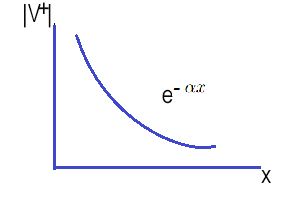
\includegraphics[width=0.7\linewidth]{./graphics/VversusXcurve}
\caption{The amplitude versus distance plot}
\label{fig:VversusXcurve}
\end{figure}

From figure~\ref{fig:VversusXcurve}, $\alpha$ is a parameter that measures how fast amplitude decay occurs in the transmission line wave. This quantity $\alpha$ is called the \emph{attenuation constant}\index{attenuation constant}. The attenuation constant measures how the wave attenuates (reduces in its value) as it travels along the structure. So it is measured in Nepers/meter.
\begin{align*}
\text{Attenuation constant,}\ \alpha = \frac{Nepers}{meter}
\end{align*}

If $\alpha$ = 1(Nepers/meter)\footnote{

\includegraphics[scale=0.2]{./graphics/johnnapier2}

The unit's name is derived from the name of John Napier. John Napier of Merchiston (1550 – 4 April 1617); also signed as Neper, Nepair; nicknamed Marvellous Merchiston, was a Scottish landowner known as a mathematician, physicist, and astronomer. He is best known as the discoverer of logarithms, he also invented the so-called \textquotedblleft Napier's bones\textquotedblright
}, then the voltage value will reduce from its initial value to $\frac{1}{e}$ for a distance x = 1 meter. So \emph{$\alpha$ relates the distance over which the amplitude drops to $\frac{1}{e}$ of its initial value}. This length at which we get $\frac{1}{e}$ is called the \emph{characteristic length}\index{characteristic length}. 

So, a distance $x = \frac{1}{\alpha}$ describes the effective travel distance in the transmission line beyond which the amplitude drops below $\frac{1}{e}$ of its initial value. Since the wave is reducing to $\frac{1}{e}$ of its initial value, the power of the wave also reduces. Taking the ratio of the initial amplitude and final amplitude after the effective travel distance we have,
\begin{align*}
\frac{\lvert V^+\rvert}{\lvert V^+\rvert e ^{-\alpha x}}
\end{align*}
Because the initial amplitude at $x = 0$ is $\left| V^+\right|$, with $x = \frac{1}{\alpha},$ the expression reduces to $\frac{1}{e}$.

We would now proceed to express the attenuation constant in decibels per metre $\left(\frac{\text{dB}}{\text{metre}}\right)$\footnote{
This is the unit in which the attenuation constant is given in most data sheets
}.
\begin{dmath*}
dB = -20\log_{10}\left(\frac{1}{e^{\alpha x}}\right)
= -20\log_{10}(e^{-\alpha x})\quad\text{With }\alpha\text{ = }1(\text{Neper/metre})\text{ and }x\text{ = }1m
= -20\log_{10}(e^{-1})
= 8.68\ dB/m 
\end{dmath*}
Therefore, 1 Neper/metre = 8.68 dB/m.

As in propagation constant $\gamma$, the attenuation constant $\alpha$ depends on the primary constant of the transmission line as well as the frequency of operation $\omega$. In general, the propagation constant $\gamma$ which is a combination of phase constant $\beta$ and attenuation constant $\alpha$ is a function of primary line parameters and frequency of operation. Hence as $\omega$ increases, $\alpha$ increases. This is the reason some structures which were satisfactorily good conductors, at low frequencies become bad conductors at high frequencies (i.e the conductor becomes a more lossy line at high frequencies).

\begin{exmp}
\subsubsection*{Measure the propagation constant}
Let R = 0.5 $\Omega$ /m, L = 0.2$\mu$H /m, C = 100pF/m, G = 0.1 $\Omega$ /m, freq = 1GHz. Calculate the propagation constant, attenuation constant and phase constant for this line.

\subsubsection*{Solution}
\[ \gamma = \sqrt{(R+\jmath\omega L)(G + \jmath\omega C)}\]
But,$ \ \omega = 2\pi f\quad$ and $\quad f = 1\textnormal{GHz} = 1 \times 10^9 \textnormal{Hz} $ 
\[\omega = 2\pi \times 10^9\textnormal{rad/s}\]
Substituting into the $ \gamma $ expression;
\[\gamma = \sqrt{(0.5 + \jmath 400\pi)(0.1 + \jmath 0.2\pi)}\]
Expanding,
\[ = \sqrt{0.5(0.1) + 0.5(\jmath 0.2\pi) + \jmath 400\pi(0.1) + \jmath 400\pi(\jmath 0.2\pi)}\]
Recall  that, $ \jmath \times \jmath = \sqrt{-1} \times \sqrt{-1} = (\sqrt{-1})^2 = -1 $
\begin{dmath*}
=\sqrt{0.05 + \jmath 0.31416 +\jmath 125.6637 - 789.568}
= \sqrt{-789.518 + \jmath 125.97786}
\end{dmath*}

We are now faced with the challenge of finding the square root of a complex number.

To find the square root, we apply \footnote{
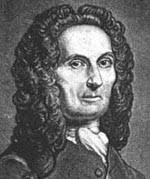
\includegraphics[scale=0.3]{./graphics/demoivre}

Named after Abraham de Moivre (26 May 1667 – 27 November 1754). He was a French mathematician known for de Moivre's formula, a formula that links complex numbers and trigonometry, and for his work on the normal distribution and probability theory. He was a friend of Isaac Newton, Edmond Halley, and James Stirling.
}DeMoivre's theorem. It states; 
\begin{equation*}
Z^{\frac{1}{n}} = |Z|^{\frac{1}{n}}\angle\frac{\theta}{n}
\end{equation*}

We first convert the complex number to polar form, that is,
\begin{equation*}
-789.518 + \jmath 125.9778 = 799.5055\angle 170.934^o
\end{equation*}
Thus,
\begin{dmath*}
\gamma = \sqrt{-789.518 + \jmath 125.9778}
= \sqrt{799.5055}\angle {\frac{170.934}{2}}^o
=28.2\angle 85.467^o
\end{dmath*}
Converting back to cartesian form, we have the propagation constant as $\gamma=2.23 +\jmath 28.1$.

This give that attenuation constant, $\alpha = 2.23467 $ Nepers/m and phase constant, $ \beta = 28.1871 $ rad/m

We now convert the attenuation constant to dB/m, thus,
\begin{align*}
1 \text{Nepers/metre} = 8.68dB/m\\
\Rightarrow 2.23467 \text{Nepers/metre} = 19.3969 dB/m
\end{align*}
\end{exmp} 

\begin{exmp}
\subsubsection*{Determine the forward traveling wave}\label{exmp:forward}
From previous example, say at x = 0, t = 0, V = 8.66V. Find the voltage at x = 1 and t = 100ns at point B as shown in figure~\ref{fig:tl} on the transmission line. Also, find the peak voltage at x = 1m. Assume the wave travels from left to right, and the initial phase $\phi = 30^o$.\\
If the wave travels from right to left, find the voltage at B.
\begin{figure}[h]
\centering
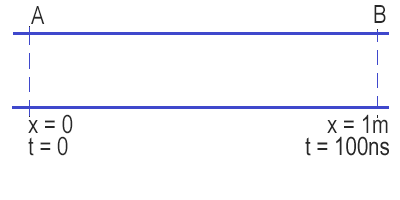
\includegraphics[width=1\linewidth]{./graphics/TL}
\caption{The transmission line showing points A and B}
\label{fig:tl}
\end{figure}

\subsubsection*{Solution}
At x = 1, the voltage is maximum, at x = 0 i.e A, V = 8.66v. Due to the direction of wave travel, we expect its amplitude to reduce to a smaller value at B. The expression
\begin{align}
V(x,t) = \mathfrak{Re}\{\left| V^+\right|  e^{-\alpha x}.e^{-\jmath\beta x + \jmath\omega t}.e^{+\jmath\phi}\} 
\label{eqn:voltagelec3soln}
\end{align}
represents the forward traveling or progressive wave moving along the +x direction.\\
Extracting the real part and including the initial phase.
\begin{align*}
V(x,t) = \lvert V^+\rvert\cos(\phi + \omega t - \beta x)e^{-\alpha x}
\end{align*}
\begin{figure}[h]
\centering
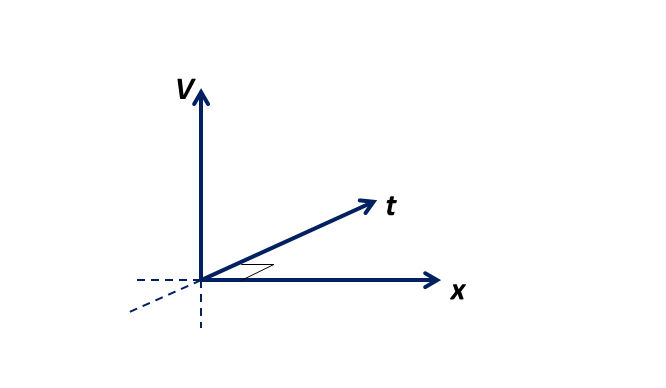
\includegraphics[width=1\linewidth]{./graphics/fig3.3}
\caption{Voltage versus distance with time}
\end{figure}

$\lvert V^+\rvert e^{-\alpha x} $ gives the amplitude variation with distance $ x $. \\
$ \phi + \omega t - \beta x $ gives the phase (including the initial phase $ \phi $).

Substituting x = 0, t = 0, and $\phi = 30^o$ into equation~\ref{eqn:voltagelec3soln},
\begin{align*}
V(x,t) &= V(0,0) = 8.66V \\
V(x,t) &= \lvert V^+\rvert\cos(\phi + \omega (0) - \beta (0))e^{-\alpha (0)}\\
8.66 &= \lvert V^+\rvert\cos(\phi)\\
8.66 &= \lvert V^+\rvert\cos(30)\\
\lvert V^+\rvert &= 10V
\end{align*}
Substituting x = 1m, t = 100ns, and $\phi = 30^o$ into equation~\ref{eqn:voltagelec3soln},\\\\
\begin{dmath*}
V(x,t) = 10\cos(\frac{\pi}{6} + 2\pi \times 10^9\times 100\times 10^{-9} - 28.18\times 1)e^{-2.235\times 1}
= 10 \times -0.815 \times e^{-2.235}
= -0.872V
\end{dmath*}
To find the peak voltage at x = 1,
\begin{align*}
V(1,t) = 10\cos(\frac{\pi}{6} + 2\pi \times 10^9t - 28.18)e^{-2.235}
\end{align*}
But the value is maximum when $\cos(\frac{\pi}{6} + 2\pi \times 10^9t - 28.18) = 1$, 
\begin{align*}
V_{\max} &= 10e^{-2.235}\\
V_{\max} &= 1.07528V
\end{align*}
We observe from the solution that attenuation took place since the amplitude reduced from 8.66V to -0.88V.

If the wave travels from right to left
\begin{dmath*}
V (x,t) = \mathfrak{Re}\{V^+ e^{+\alpha x}.e^{+\jmath\beta x + \jmath\omega t}e^{+\jmath\phi}\}
= \lvert V^+\rvert\cos(\phi + \omega t + \beta x)e^{+\alpha x}
= 10\cos(\frac{\pi}{6} + 2\pi\times10^9\times100\times10^{-9} + 28.18\times1) e^{+2.235\times1}
= 10 \times-0.9093 \times e^{+2.235}
= -84.99V
\end{dmath*}
This is the amplitude of the voltage at point B that will undergo attenuation in moving backwards from B to A.	
\end{exmp}

\begin{exmp}
\subsubsection*{Determine the backward traveling wave}
Given that the wave in the previous example is travelling in the negative ${x}$ direction and all other parameters are kept the same, what is the instantaneous voltage at the same time and at the same location?

\subsection*{Solution}
\begin{figure}[h]
\centering
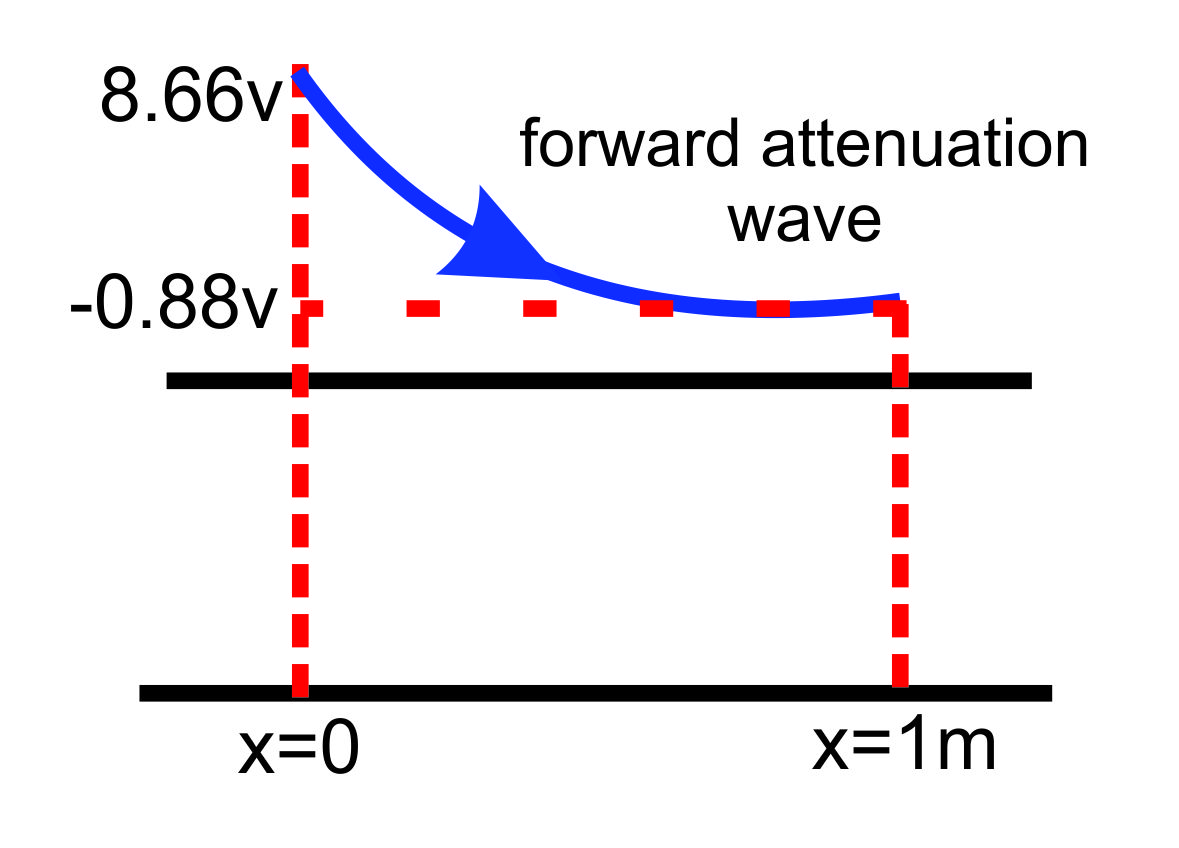
\includegraphics[scale=0.5]{./graphics/Group98}
\caption{Solution for example \ref{exmp:forward}}
\label{fig:group98}
\end{figure}

For the wave travelling in the negative direction, we have $V_{(x,t)} = \mathfrak{Re}\left\lbrace V^{-}e^{\gamma x}e^{j\omega t}\right\rbrace$ for backward wave.
\begin{dmath*}
V(x,t) = \mathfrak{Re}\left\lbrace{V^{-}e^{\alpha x}e^{j\beta x}e^{j\omega t}}\right\rbrace = |V^{-}|e^{\alpha x}cos{(\phi+\omega t + \beta x)}
\end{dmath*}
At ${t=0, x=0, V=8.66}$, then
\begin{dmath*}
{8.66} = {|V^{-}|}e^{0} cos({\phi + 0 + 0})
= {|V^-|{cos\phi}} \quad \text{at }\phi\text{= 30\textdegree} 
= {|V^-|{cos30}}
= {|V^-|{0.866}}
\end{dmath*}
\begin{dmath*}
\frac{8.66}{0.866} = {|V^-|} = 10V
\end{dmath*}
\begin{align*}
V({x,t}) = 10e^{2.23x} \cos({\dfrac{\pi}{6} + 2\pi\times10^9t + 28.2x})
\end{align*}
At ${t=100nsec}$ and ${x=1m}$
\begin{dmath*}
V({x,t}) = 10e^{2.23} \cos({\dfrac{\pi}{6} + 2\pi\times10^9\times100\times10^{-9} + 28.2})
= -83.7701V
\end{dmath*}
So what we note here is, if we look at the transmission line with ${x=0}$ and ${x=1m}$. If the wave travels in forward direction, then the wave will attenuate in the direction of propagation. The variation is from ${8.66V}$ to ${-0.88V}$. In the backward direction, the wave will attenuate in the reverse direction so it has to  have a higher amplitude at ${x=1m}$ and ${t=100nsec}$ from were it attenuates from ${-83.7701V}$ to ${8.66V}$ in the other direction. The direction of propagation of the wave is very important.
\end{exmp}
    
% \begin{exmp}
% Let R = 0.4 $\Omega$ /m, L = 0.3$\mu$H /m, C = 120pF/m, G = 0.08 $\Omega$ /m, freq = 1GHz. Calculate the propagation constant, attenuation constant and phase constant for this line.

% \subsubsection*{Solution}
% \[\gamma = \sqrt{(R+\jmath\omega L)(G + \jmath\omega C)}\]
% But, $\omega = 2\pi f\quad$ and $\quad f = 1GHz = 1 \times 10^9 $ Hz
% \[\omega = 2\pi \times 10^9rad/s.\]
% Substituting into the $\gamma$ expression; 
% \begin{dmath*}
% \sqrt{0.4+\jmath(2\pi\times10^9)\times0.3\times10^{-6}}\times\sqrt{0.08+\jmath(2\pi\times10^9) \times120 \times10^{-12}} 
% \end{dmath*}
% \begin{dmath*}
% \gamma=\sqrt{(0.5+\jmath600\pi) (0.08+\jmath0.24\pi)}
% = \sqrt{0.4(0.08) + 0.4(\jmath0.24\pi) + \jmath600\pi(0.08) + \jmath600\pi(\jmath0.24\pi)}
% \end{dmath*} 
% Recall  that,$ \quad \jmath \times \jmath = \sqrt{-1} \times \sqrt{-1} = (\sqrt{-1})^2 = -1$

% Thus,
% \begin{dmath*}
% \gamma =\sqrt{0.032 + \jmath 0.3016 +\jmath 150.7964 - 1421.2230} = \sqrt{-1421.191 + \jmath 151.098} 
% \end{dmath*}

% We first convert the complex number to polar form, thus:
% \[-1421.191 + \jmath 151.098 = 1429.2006\angle 173.931^o\]
% \begin{dmath*} 
% \sqrt{-1421.191 + \jmath 151.098} = \sqrt{1429.2006}\angle \frac{173.931}{2}
% =37.8\angle 86.9655 
% \end{dmath*}
% Converting back to cartesian form;
% \[\textnormal{Propagation constant,}\quad\gamma=2 +\jmath 37.747\]
% From the expression; $ \alpha = 2 $ Nepers/m, $ \beta = 37.747 $ rad/m.

% We now convert the attenuation constant to dB/m (1 Nepers/m = 8.68dB/m), thus, 2 Nepers/m = 17.36 dB/m.
% \end{exmp} 

\section{The Characteristic Impedance}\index{characteristic impedance}
As derived in equations~\eqref{eqn:deltav} and~\eqref{eqn:deltai}
\begin{align}
\frac{dV}{dx} = -(R+\jmath\omega L)I\label{eqn:deltavlec3}\\
\frac{dI}{dx} = -(G+\jmath\omega C)V\label{en:deltavlec3}
\end{align}
Also, the volatage wave solution derived in equation~\eqref{eqn:solnv} is given and the same can be written for the current wave equation as follows
\begin{align*}
V = V^+e^{-\gamma x}+V^-e^{+\gamma x}\\
I = I^+e^{-\gamma x}+I^-e^{+\gamma x}
\end{align*}
Substituting $V$ and $I$ into the differential equation~\eqref{eqn:deltavlec3},
\[
\frac{d}{dx}(V^+e^{-\gamma x}+V^-e^{+\gamma x}) = -(R+\jmath\omega L)(I^+e^{-\gamma x}+I^-e^{+\gamma x})
\]
Thus,
\[
-\gamma V^+e^{-\gamma x}+\gamma V^-e^{+\gamma x} = -(R+\jmath\omega L)(I^+e^{-\gamma x}+I^-e^{+\gamma x})
\]
$(V^+,I^+)$ represents the forward traveling waves, while $(V^-,I^-)$ represents the backward traveling waves for voltage and current respectively. The relationship between voltage and current has to be satisfied at every point along the transmission line. This will happen if and only if
\begin{align*}
-\gamma V^+e^{-\gamma x} = -(R+\jmath\omega L)I^+e^{-\gamma x}
\end{align*}
So,
\begin{align}
\frac{V^+}{I^+} = \frac{R+\jmath\omega L}{\gamma}
\label{eqn:voveriforward}
\end{align}
Similarly, for the backward traveling wave, 
\begin{align*}
\gamma V^-e^{+\gamma x} = -(R+\jmath\omega L)I^-e^{+\gamma x}
\end{align*}
So,
\begin{align}
\frac{V^-}{I^-} = -\frac{R+\jmath\omega L}{\gamma}
\label{eqn:voveribackward}
\end{align}
The equations~\eqref{eqn:voveriforward} and~\eqref{eqn:voveribackward} show the relationship between forward and backward traveling waves for voltage and current.

Recall that $\gamma = \sqrt{(R + \jmath\omega L)(G + \jmath\omega C)}$, therefore from equation~\eqref{eqn:voveriforward}
\begin{dmath}
\frac{V^+}{I^+} = \frac{R+\jmath\omega L}{\sqrt{(R + \jmath\omega L)(G + \jmath\omega C)}}
= \frac{\sqrt{(R+\jmath\omega L)^2}}{\sqrt{(R + \jmath\omega L)(G + \jmath\omega C)}}
=\sqrt{\frac{(R+\jmath\omega L)(R+\jmath\omega L)}{(R + \jmath\omega L)(G + \jmath\omega C)}}
=\sqrt{\frac{R+\jmath\omega L}{G+\jmath\omega C}}
\label{eqn:voveriforward2}
\end{dmath}
Similarly for equation~\eqref{eqn:voveribackward}
\begin{dmath}
\frac{V^-}{I^-} = \frac{-(R+\jmath\omega L)}{\sqrt{(R + \jmath\omega L)(G + \jmath\omega C)}}
=-\sqrt{\frac{R+\jmath\omega L}{G+\jmath\omega C}}
\label{eqn:voveribackward2}
\end{dmath}
The expression $\sqrt{\frac{R+\jmath\omega L}{G+\jmath\omega C}}$ is another characteristic of the transmission line since it depends only on the primary constants and the frequency of operation. Also, this parameter is the ratio of voltage and current and as such has a definition of impedance. Hence the reason it is called the \emph{characteristic impedance} of the line and it is denoted by $Z_0$. Thus,
\begin{equation}
Z_0 = \sqrt{\frac{R+\jmath\omega L}{G+\jmath\omega C}}
\label{eqn:xteristicimp}
\end{equation}
The characteristic impedance, $Z_0$ governs energy flow on the transmission line and will be discussed later in this chapter. So these two parameters, the propagation constant $\gamma$ and the characteristic impedance $Z_0$ completely characterize the propagation of wave along a transmission line. Though $R$, $L$, $G$ and $C$ are the primary constants, they are hardly given in any transmission line problem. Instead, a transmission line is characterized by its propagation constant $\gamma$ and characteristic impedance $Z_0$. These values are usually given in the datasheet of transmission lines and this is sufficient information to solve any transmission line problem.

From equations~\eqref{eqn:voveriforward2} and~\eqref{eqn:voveribackward2}, substituting for equation~\eqref{eqn:xteristicimp} we can write
\begin{align}
\frac{V^+}{I^+} &= Z_0\\
\frac{V^-}{I^-} &= -Z_0
\end{align}
These show that at any point on the transmission line, the ratio of voltage to current (forward or backward) is always constant i.e equal to characteristic impedance. Hence a forward traveling wave sees an impedance of $Z_0$ and the reverse traveling wave sees an impedance of $-Z_0$. If $Z_0$ is real, it means the forward traveling wave sees a positive resistance while the backward traveling wave sees a negative resistance.

But, \emph{what does a negative resistance mean?} Ordinarily, energy flow is from the generator to the load which the positive resistance represents. The negative resistance means energy is being carried backwards i.e energy is flowing from the load into the generator.

In conclusion, irrespective of the boundary condition of the transmission line, the forward traveling wave always sees an impedance equal to the characteristic impedance while a backward traveling wave sees a negative of the characteristic impedance.

We have thus established that;
\begin{align*}
\frac{V^+}{I^+} = Z_0,\quad I^+ = \frac{V^+}{Z_0}\quad\text{and}\\
\frac{V^-}{I^-} = -Z_0,\quad I^- = -\frac{V^-}{Z_0}
\end{align*}
Therefore, we can now rewrite the voltage and current wave equations as
\begin{align}
V &= V^+e^{-\gamma x}+V^-e^{+\gamma x}
\label{eqn:voltagelec3}\\
I &= \frac{V^+}{Z_0}e^{-\gamma x}-\frac{V^-}{Z_0}e^{+\gamma x}
\label{eqn:currentlec3}
\end{align}

\section{Boundary Conditions}
Up until now, we have not defined the boundary conditions of the transmission line, so let us discuss that in this section. We have two spatial locations on the transmission line, one at the generator and the other where an arbitrary load $Z_L$ is connected as shown in figure~\ref{fig:tlcircuit}.
\begin{figure}[h]
\centering
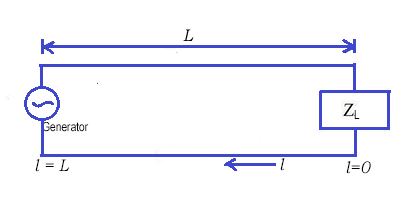
\includegraphics[scale=0.8]{./graphics/tlcircuit}
\caption{The transmission line showing generator and load}
\label{fig:tlcircuit}
\end{figure}

To define boundary conditions, we define the spatial distance from the load end, the origin, so that all distances move from the load end towards the generator. So we now have a parameter that moves towards the generator from the load side. At the load point $l = 0$ and at the generator, $l = L$. So $l = -x$ in our transmission line equations, therefore, substituting $l = -x$ in equations~\ref{eqn:voltagelec3} and~\ref{eqn:currentlec3}, we have
\begin{align}
V &= V^+e^{+\gamma l}+V^-e^{-\gamma l}
\label{eqn:voltagefromload}\\
I &= \frac{V^+}{Z_0}e^{+\gamma l}-\frac{V^-}{Z_0}e^{-\gamma l}
\label{eqn:currentfromload}
\end{align}
Beyond this point all of our analysis will be done using the wave equations~\eqref{eqn:voltagefromload} and~\eqref{eqn:currentfromload}

\section{The Reflection Coefficient}\index{reflection coefficient}
At $l = 0$, $Z = Z_L$ since $Z_L$ terminates the transmission line at this point. Substituting $l = 0$ into Equations~\eqref{eqn:voltagefromload} and~\eqref{eqn:currentfromload},
\begin{align*}
V &= V^+e^{+\gamma (0)}+V^-e^{-\gamma (0)} = V^+ + V^-\\
I &= \frac{V^+}{Z_0}e^{+\gamma (0)}-\frac{V^-}{Z_0}e^{-\gamma (0)} = \frac{V^+}{Z_0} - \frac{V^-}{Z_0} \\
I &= \frac{V^+ - V^-}{Z_0}
\end{align*}
\begin{align*}
\frac{V}{I} = \left( \frac{V^+ + V^-}{1}\right)  \times \left( \frac{Z_0}{V^+ - V^-}\right) 
\end{align*}

\begin{equation*}
Z_{L} = \frac{V}{I}\left|_{l = 0} = Z_0 \left[ \frac{V^+ + V^-}{V^+ - V^-} \right]\right.    
\end{equation*}
Thus,
\begin{equation}
Z_L = Z_0 \left[\frac{V^+ + V^-}{V^+ - V^-} \right]
\end{equation}
It is clear from the equation that the load impedance is related to the characteristic impedance and also related to the amplitude of the forward and backward waves. We can simplifiy further by dividing the top and bottom by $V^+$, then
\begin{dmath}
Z_L = Z_0\left[ \frac{\frac{V^+ + V^-}{V^+}}{\frac{V^+ - V^-}{V^+}}\right]
= Z_0\left[ \frac{1+ \frac{V^-}{V^+}}{1 - \frac{V^-}{V^+}}\right] 
\label{eqn:impedatload}
\end{dmath}
Here we see that the absolute values of $V^+$ and $V^-$ do not matter, instead, the ratio $\frac{V^-}{V^+}$ is what's important. Hence we define a new parameter on which $Z_L$ depends. This parameter is known as the \emph{reflection coefficient}. It can be defined as the ratio of backward traveling wave to forward traveling wave on the transmission line.

The reflection coefficient is denoted by $\Gamma$\footnote{
$\Gamma$ is capital Gamma, the third letter of the Greek alphabet.
}.
\begin{align*}
\Gamma = \frac{\text{Backward traveling wave}}{\text{Forward traveling wave}}
\end{align*}
\begin{align}
\Gamma(l) = \frac{V^-e^{-\gamma l}}{V^+e^{+\gamma l}}
\label{eqn:rfc}
\end{align}
$\Gamma(l)$ is the reflection coefficient at any point on the line.

At $l = 0$,
\begin{dmath}
\Gamma (0) = \frac{V^-e^{-\gamma (0)}}{V^+e^{+\gamma (0)}}
= \frac{V^-}{V^+}
= \Gamma_L
\label{eqn:rfcatload}
\end{dmath}
$\Gamma_L$ is the reflection coefficient at the load point on the line and it will be used to represent the reflection coefficient at the load point from the point onwards.

Substituting equation~\eqref{eqn:rfcatload} into equation~\eqref{eqn:rfc},
\begin{equation*}
\Gamma (l) = \Gamma_L\frac{e^{-\gamma l}}{e^{+\gamma l}}
\end{equation*}
\begin{equation}
\Gamma (l) = \Gamma_L e^{-2\gamma l}
\label{eqn:rfc2}
\end{equation}
Recall, equation~\ref{eqn:impedatload} was derived at the load point. We would now derive the relationship at any point on the line.

Dividing Equation~\eqref{eqn:voltagefromload} by equation~\eqref{eqn:currentfromload},
\begin{align*}
\frac{V}{I} &= \frac{V^+e^{+\gamma l}+V^-e^{-\gamma l}}{1}\times \frac{Z_0}{V^+e^{+\gamma l}-V^-e^{-\gamma l}}\\
&= Z_0\left( \frac{V^+e^{+\gamma l}+V^-e^{-\gamma l}}{V^+e^{+\gamma l}-V^-e^{-\gamma l}}\right) 
\end{align*}
Dividing top and bottom by $V^+e^{+\gamma l}$
\begin{dmath*}
\frac{V}{I} = Z_0\left( \frac{\dfrac{V^+e^{+\gamma l}}{V^+e^{+\gamma l}}+\dfrac{V^-e^{-\gamma l}}{V^+e^{+\gamma l}}}{\dfrac{V^+e^{+\gamma l}}{V^+e^{+\gamma l}}-\dfrac{V^-e^{-\gamma l}}{V^+e^{+\gamma l}}}\right)
= Z_0\left( \frac{1 + \dfrac{V^-e^{-\gamma l}}{V^+e^{+\gamma l}}}{1 - \dfrac{V^-e^{-\gamma l}}{V^+e^{+\gamma l}}}\right)\quad\text{From Equation~\ref{eqn:rfc}}
=Z_0\left( \frac{1+\Gamma (l)}{1 -\Gamma (l)}\right)
\end{dmath*}
Substituting for $\Gamma (l)$ from equation~\eqref{eqn:rfc2}, we have the expression at any point on the line.
\begin{equation}
Z(l) = Z_0\left[ \frac{1 + \Gamma_L e^{-2\gamma l}}{1 - \Gamma_L e^{-2\gamma l}}\right] 
\end{equation}
At $l = 0$ 
\begin{dmath}
Z_L = Z_0\left[ \frac{1 + \Gamma_L e^{-2\gamma (0)}}{1 - \Gamma_L e^{-2\gamma (0)}}\right] 
= Z_0\left[\frac{1 + \Gamma_L}{1 - \Gamma_L}\right] 
\end{dmath}
\begin{align*}
Z_L(1 - \Gamma_L) &= Z_0(1 + \Gamma_L)\\
Z_L - Z_0 &= (Z_0 + Z_L)\Gamma_L
\end{align*}
\begin{equation}
\Gamma_L = \frac{Z_L - Z_0}{Z_L + Z_0}
\label{eqn:reflectioncoefficientatload}
\end{equation}
The reflection coefficient in equation~\eqref{eqn:reflectioncoefficientatload} decribes the ratio between reflected and incident voltage. \emph{It is a measure of how much energy is reflected from the transmission line and is related to the terminating impedance of the line and the characteristic impedance.}

\section*{Exercises}
\begin{ExerciseList}
\Exercise[label={ex31}]
With appropriate equation of amplitude variation along a transmission line, explain what is meant by Characteristic length.

\Exercise[label={ex32}]
In what unit is attenuation constant stated in most data sheets?

\Exercise[label={ex33}]
Starting from the differential equation guilding transmission lines, derive the characteristic impedance relation. What does negative impedance imply from the backward voltage to current ratio?

\Exercise[label={ex34}]
What are the physical significance of the propagation constant($\gamma$), attenuation constant($\alpha$) and phase constant($\beta$)?

\Exercise[label={ex35}]
Let $R = 0.4\varOmega$/m, $L = 0.3\mu$H/m, $C = 120$pF/m, $G = 0.08\varOmega$/m, and $f = 1$GHz. Calculate the propagation constant, attenuation constant and phase constant for this line.

\Answer[ref={ex35}]
(a) Propagation constant, $\gamma = 2 +\jmath 37.747$ (b)Attenuation constant, $\alpha = 2$ Nepers/m (17.36 dB/m) (c) Phase constant, $\beta = 37.747 $ rad/m.

\Exercise[label={ex36}]
From $ V = V^+e^{+\lambda l} + V^-e^{-\lambda l} $ and $ I = \frac{V^+}{Z_0}e^{+\lambda l} - \frac{V^-}{Z_0}e^{-\lambda l}$, show that $ \Gamma_L = \frac{Z_L - Z_0}{Z_L + Z_0} $.
\end{ExerciseList}